\documentclass[11pt]{article}

%%%%%%%%%%%%%%%%%%%%%%%%%%%%%%%%%%%%%%%%%%%%%%%%%%%%%%%%
% Imports 		%%%%%%%%%%%%%%%%%%%%%%%%%%%%%%%%%%%%%%%%
%%%%%%%%%%%%%%%%%%%%%%%%%%%%%%%%%%%%%%%%%%%%%%%%%%%%%%%%

	\usepackage{amsmath,amsfonts,amsthm,amssymb,amsopn,bm} %%% load AMS-Latex Package
	\usepackage{graphics,graphicx,subfigure,color} %figures and color	

	%%% paper layout, stylistic etc
	\usepackage{epsfig,fullpage}
	\usepackage{url}
	\usepackage[pdfborder={0 0 1}, colorlinks=true, citecolor=black, plainpages=false]{hyperref}
	\usepackage{parskip} %dont indent paragraphs
	\usepackage[makeroom]{cancel}


	\usepackage{tikz} % graphical models
	\usetikzlibrary{chains,fit,shapes}
	\usetikzlibrary{bayesnet}

%%%%%%%%%%%%%%%%%%%%%%%%%%%%%%%%%%%%%%%%%%%%%%%%%%%%%%%%
% Commands 		%%%%%%%%%%%%%%%%%%%%%%%%%%%%%%%%%%%%%%%%
%%%%%%%%%%%%%%%%%%%%%%%%%%%%%%%%%%%%%%%%%%%%%%%%%%%%%%%%

	\newcommand{\vct}[1]{\boldsymbol{#1}} % vector
	\newcommand{\mat}[1]{\boldsymbol{#1}} % matrix
	\newcommand{\cst}[1]{\mathsf{#1}} % constant
	\newcommand{\T}{^{\textrm T}} % transpose

	\newcommand{\inner}[2]{#1\cdot #2}
	\newcommand{\norm}[1]{\left\|#1\right\|}
	\newcommand{\twonorm}[1]{\|#1\|_2^2}

	\newcommand{\ProbOpr}[1]{\mathbb{#1}} % hollow letter
	\newcommand{\SetOf}[1]{\mathbf{#1}} % Capital set bold letter


	\newcommand{\cind}[3]{{#1} \independent{#2}\,|\,#3}  % conditional independence
	\newcommand{\cndexp}[2]{\ProbOpr{E}\,[ #1\,|\,#2\,]} % conditional expectation

	\newcommand{\degrees}[1]{#1$^{\circ}$} % degrees
	\newcommand{\prob}[1]{\text{p}(#1)} % probability
	\newcommand{\entropy}[1]{\text{H}[#1]} % entropy


	\DeclareMathOperator*{\argmin}{argmin}
	\DeclareMathOperator*{\argmax}{argmax}

	\newcommand{\Eq}[1]{\begin{align*}#1\end{align*}} % conditional expectation

	\newcommand{\italic}[1]{\textit{#1}} % italic
	% \newcommand{\bold}[1]{\textbf{#1}} % bold

%%%%%%%%%%%%%%%%%%%%%%%%%%%%%%%%%%%%%%%%%%%%%%%%%%%%%%%%
% Document 		%%%%%%%%%%%%%%%%%%%%%%%%%%%%%%%%%%%%%%%%
%%%%%%%%%%%%%%%%%%%%%%%%%%%%%%%%%%%%%%%%%%%%%%%%%%%%%%%%

\title{PGM Interactive Object Recognition Project}
\author{Chet Corcos, Karol Hausman, Timmy Mbaya }
\begin{document}

\maketitle
\tableofcontents

\newpage

\section{Introduction}

	The goal of this project is to create an object recognition algorithm that determines optimal actions for recognition. We will train our model on a variety of objects in a variety of poses with known actions between the poses, measuring/extracting/computing a variety of features. Certain features associated with an object may only be visible in a certain pose. The model in this document will be a simplified model with discrete poses. Future work can incorporate continuous pose and action variables.
\section{Related Work}

	Research in perception has traditionally focused on  static 
	images and recognized objects based on a set of visual features  such as SIFT~\cite{lowe2004distinctive}, SURF~\cite{bay2006surf} or ORB~\cite{rublee2011orb}.
	There has also been plethora of work on static object recognition that resulted in various systems.
	
	One of the most efficient and robust object recognition systems was developed by Tang et al.~\cite{tang2012textured}. It is worth mentioning that the system took the 1st place in the ICRA 2011 Solutions in Perception instance recognition challenge. The system can be divided into several steps. In the training phase a full object model is created, then it is transformed into a mesh, and finally, the RGB data is projected onto the object model acquired in the previous steps. The authors decided to use SIFT features and color histograms in order to fully describe the textural property of the object. In the testing phase plane extraction and euclidean clustering algorithms are employed in order to segment the object. As next steps color model matching and SIFT feature matching are used to recognize the object. The algorithm also performs geometric pose estimation as well as final scene verification and refinement using global scene consistency checks. 

	A different approach was discussed by Weijer and Khan~\cite{van2013fusing} where the authors compare various bag-of-words based recognition algorithms. The algorithm represents an image as a set of local regions where each of them is represented as a visual vocabulary. Different objects correspond to different histograms (called bags-of-words) over the created vocabulary. An extracted bag-of-words histogram can be compared to all the histograms stored in the memory and thus, an object can be labelled as one of the previously seen objects. 

	Although the above mentioned methods are established as the state-of-the-art object recognition systems, we still cannot say that the problem of object recognition has been solved. We claim that the reason for that is already included in the problem formulation. Given static images there are cases where it is impossible to recognize the object simply because of lack of distinctive features. One way to overcome this problem has been presented in the area of object segmentation where robot-objects interaction was introduced.

	Segmentation of rigid objects from a video stream 
	of objects being moved by a robot has been first addressed by Fitzpatrick et. al.~\cite{fitzpatrick_active_vision} and Kenney et. al.~\cite{KenneyInteractive}.
	Katz and Brock~\cite{Katz-WS-MM-ICRA2011} address
	the problem of segmenting the articulated objects. Another technique was presented by \cite{bergstrom11icvs}, where the authors propose  an   approach  to
	interactive  segmentation that  requires initial  labeling using  a 3D
	segmentation  through  fixation  which  results  in  a  rough  initial
	segmentation. The robot interacts with the scene to disambiguate
	the hypotheses.

	All these approaches do not take into consideration action choices, action is assumed to be known and performed either by a human or a robot. In our approach we tackle interactive object recognition problem but we look for the action that will minimize the entropy over objects distribution. Therefore we want to be optimal in the number of actions that will lead us to successful object recognition.





	There are two especially ambiguous recognition cases to consider in evaluating this algorithm. 
\section{Example cases}

	There are two especially ambiguous recognition cases to consider in evaluating this algorithm. 
\subsection{Book Ambiguity}

	Suppose there are two similar books with different covers. If you are observing a one of the books upside-down, we do not know which book it is. However we know that the most discriminative features between these books will be exposed if we flip the book over, and thus that is the optimal action.
\subsection{Ball Ambiguity}

	Suppose there are two very similar textureless balls, except one ball has a mark on it. The pose of the unmarked ball is always ambigious. The pose of the marked ball is only unambigious if we observe the mark. If observing a ball with no mark on it, the optimal action would be to rotate the ball through all poses until finding a mark or deducing the absense of the mark. This case requires a history of actions and observed features in order to deduce recognition of the markless ball.
\section{Recording Data}
	We will record data for $N$ objects in $I$ poses measuring $M$ features of $J$ different types. In addition to some standard household items, we will record data for ambiguous object such as the balls and books from the ambigous cases discusses earlier.

	This algorithm should work for any features provided a matching error function for the feature which will be computed. Some example features to extract:

	\begin{itemize}
	 \item SURF
	 \item Color spectrum
	 \item 3D point cloud
	\end{itemize}

	Since we do not have access to a robot arm, I propose $M=8$ poses, right-side up and up-side down, with 4 orientations \degrees{90} apart for each, $\SetOf{P}=\{p_{+0},p_{+90},p_{+180},p_{+270},p_{-0},p_{-90},p_{-180},p_{-270}\}$. This leaves $C=I-1=7$ pairwise \italic{relative} actions between poses, $\SetOf{A}=\{a_{+90},a_{+180},a_{+270},a_{-0},a_{-90},a_{-180},a_{-270}\}$.
\section{Model}

	Before considering actions, our model can be represented as a Bayesian Network (BN) where features $\SetOf{F}$ are dependent on objects $\SetOf{O}$ and poses $\SetOf{P}$. 

	\begin{center}
	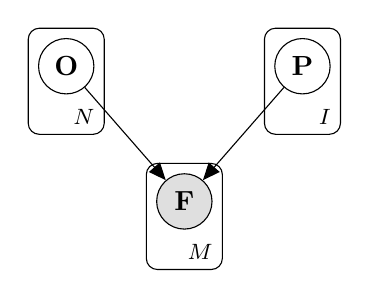
\begin{tikzpicture}
	  % Define nodes
	  \node[obs]                            (F) {$\SetOf{F}$};
	  \node[latent, above=of F, xshift=-1.5cm] (O) {$\SetOf{O}$};
	  \node[latent, above=of F, xshift=1.5cm]  (P) {$\SetOf{P}$};

	  % Connect the nodes
	  \edge {P,O} {F};

	  % Plates
	  \plate {} {(P)} {$I$}
	  \plate {} {(O)} {$N$}
	  \plate {} {(F)} {$M$}
	\end{tikzpicture}
	\end{center}

	The joint distribution:

	\Eq{\prob{\SetOf{O},\SetOf{P},\SetOf{F} } &= \prob{\SetOf{O}} \cdot \prob{\SetOf{P}}  \cdot \prob{\SetOf{F}|\SetOf{O},\SetOf{P} } }

	The posterior distribution:

	\Eq{\prob{o,p|\SetOf{F}} = \frac{\prob{o,p} \cdot \prob{\SetOf{F}|o,p}}{\prob{\SetOf{F}}}}

	posterior: $\prob{o,p|\SetOf{F}}$

	prior: $\prob{o,p} = \frac{1}{N \cdot I} = \frac{1}{K}$

	likelihood: $\prob{\SetOf{F}|o,p}$

	evidence: $\prob{\SetOf{F}}$

	Each feature type has an associated error function. In the case of SURF features, each feature has an associated descriptor which can be compared against other descriptors. In the case of a color histogram, every color histogram recorded during training gets a node on the graph, and an error function could be something like the mean-square error. A 3D point could feature could be treated the same. 

\section{Approach 1}
\subsection{Training}

	First we need to construct the graph. Every object, pose, and feature in the training data gets a node on the graph.

	Lets use a toy example to illustrate. We have two similar books in two poses. We observe 4 SURF features and 4 color histograms. When we generate our graph, we will have 8 feature nodes, 2 object nodes, and 2 pose nodes. 

	Each feature is a specific parameterization/descriptor and each feature type has a matching function that returns the error between two features. 

	Lets suppose that for the training data the observed features for each object-pose are given by

	\begin{table}[h]
		\centering
		\begin{tabular}{c} % number of columns and vertical lines
			$o_1,p_1$:  $f_1^1$, $f_5^2$ \\
			$o_1,p_2$: 	$f_2^1$, $f_6^2$ \\
			$o_2,p_1$: 	$f_3^1$, $f_7^2$ \\
			$o_2,p_2$: 	$f_4^1$, $f_8^2$ 
		\end{tabular}
	\end{table}

	The superscript represents the fact that there are two types of features: SURF and color histogram. (Only one SURF feature was found per image)

	Then, iterating through each training sample we compute the feature errors. Here is an example for the ambiguous book case where $p_1$ is the front of the book and $p_2$ is the back of the book.

	\begin{table}[h]
		% \caption{Training Errors}
		\centering
		\begin{tabular}{c|c c c c c c c c} % number of columns and vertical lines
			& $f_1^1$ & $f_2^1$ & $f_3^1$ & $f_4^1$ & $f_5^2$ & $f_6^2$ & $f_7^2$ & $f_8^2$ \\
			% [0.5ex] % [0.5ex] adds vertical space
			\hline 	    % o1 f    o1 b    o2 f    o2 b    o1 f    o1 b    o2 f    o2 b    
			$o_1,p_1$ 	& 0 	& 10 	& 9 	& 10	& 0 	& 100 	& 40 	& 100	\\
			$o_1,p_2$ 	& 10 	& 0 	& 10	& 1		& 100 	& 0 	& 100	& 2		\\
			$o_2,p_1$ 	& 8 	& 10 	& 0 	& 10	& 50 	& 100 	& 0 	& 100	\\
			$o_2,p_2$ 	& 10	& 1 	& 10	& 0 	& 100	& 1 	& 100	& 0 	
		\end{tabular}
		% \label{tab:trainingErrors}
	\end{table}

	What is represented in this table is the minimum matching error between the feature in the column, and the features observed for the training sample in the row.

	Note that the errors returned by different feature types can have vastly different scales. 

	The back of both books are ambiguous but the front of the books are not. Notice that $f_2$ and $f_6$ were observed for $o_1,p_2$ and thus the error is zero, but due to the ambiguity of the back of these books, $f_4$ and $f_8$ also have reasonably small errors.

	Lets consider taking a new observation. We observe a set of features for an unknown object-pose $o_?,p_?$ and compute the minimum matching errors between observated features and all of the features in the model, $\SetOf{F}$. 

	\begin{table}[h]
		% \caption{Training Errors}
		\centering
		\begin{tabular}{c|c c c c c c c c} % number of columns and vertical lines
			& $f_1^1$ & $f_2^1$ & $f_3^1$ & $f_4^1$ & $f_5^2$ & $f_6^2$ & $f_7^2$ & $f_8^2$ \\
			% [0.5ex] % [0.5ex] adds vertical space
			\hline 	    % o1 f    o1 b    o2 f    o2 b    o1 f    o1 b    o2 f    o2 b    
			$o_?,p_?$ 	& 9 	& 2 	& 11	& 1		& 102 	& 3 	& 100	& 4	
		\end{tabular}
		% \label{tab:trainingErrors}
	\end{table}

	Now we need to determine which feature we are observing. First, we need to know the distribution for $\prob{f|o,p}$. To do this, we need to gather a many training samples for each object pose, compute the errors, and learn a distribution.

	\begin{table}[h]
		% \caption{Training Errors}
		\centering
		\begin{tabular}{c|c c c c c c c c} % number of columns and vertical lines
			& $f_1^1$ & $f_2^1$ & $f_3^1$ & $f_4^1$ & $f_5^2$ & $f_6^2$ & $f_7^2$ & $f_8^2$ \\
			% [0.5ex] % [0.5ex] adds vertical space
			\hline 	    % o1 f    o1 b    o2 f    o2 b    o1 f    o1 b    o2 f    o2 b    
			$o_1,p_1$ 	& 1 	& 10 	& 9 	& 9	& 2 	& 102 	& 42 	& 98	\\
			$o_1,p_1$ 	& 2 	& 8 	& 11 	& 11	& 2 	& 101 	& 40 	& 101	\\
			$o_1,p_1$ 	& 1 	& 9 	& 10 	& 11	& 2 	& 99 	& 41 	& 101	\\
			$o_1,p_1$ 	& 3 	& 11 	& 10 	& 10	& 1 	& 100 	& 40 	& 100
		\end{tabular}
		\label{tab:trainingErrors}
	\end{table}

	Now, to learn $\prob{f_1^1|o_1,p_1}$, we just need to learn a distribution over the training sample errors, [1,2,1,3]. This could be a Gaussian distribution, or more rigorously a Half-normal distribution. 
\subsection{Inference}

	After an observation, we first want to compute the posterior for all object-poses.

	\Eq{\prob{o,p|\SetOf{F}} = \frac{\prob{o,p} \cdot \prob{\SetOf{F}|o,p}}{\prob{\SetOf{F}}}}

	We can do this by computing

	\Eq{\prob{\SetOf{F}|o,p} = \prod_f \prob{f|o,p}}

	\Eq{\prob{\SetOf{F}} &= \sum_{n,i} \prob{o_n,p_i,\SetOf{F}}\\
	&= \sum_{n,i} \prob{\SetOf{F}|o_n,p_i}\cdot \prob{o_n,p_i}\\
	&= \frac{1}{K} \sum_{n,i} \prob{\SetOf{F}|o_n,p_i}}

	After the observing of an object for the first time, we want to determine an optimal action which leads to a new pose and a new set of observed features. Thus, our model is actually a dynamic BN. 

	\begin{center}
	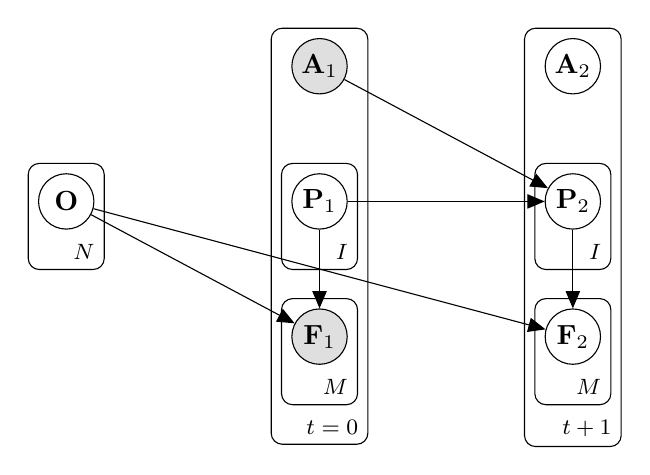
\begin{tikzpicture}
		% Define nodes
		\node[obs] (F) {$\SetOf{F}_1$};
		\node[latent, above=of F]  (P) {$\SetOf{P}_1$};
		\node[latent, left=of P, xshift=-1.5cm] (O) {$\SetOf{O}$};
		\node[obs, above=of P]  (A) {$\SetOf{A}_1$};

		\node[latent, right=of F, xshift=1.5cm] (F2) {$\SetOf{F}_2$};
		\node[latent, above=of F2]  (P2) {$\SetOf{P}_2$};
		\node[latent, above=of P2]  (A2) {$\SetOf{A}_2$};


	  % Connect the nodes
		\edge {P,O} {F};
		\edge {P2,O} {F2};
		\edge {P,A} {P2};

		% Plates
		\plate {pp} {(P)} {$I$}
		\plate {po} {(O)} {$N$}
		\plate {pf} {(F)} {$M$}

		\plate {pp2} {(P2)} {$I$}
		\plate {pf2} {(F2)} {$M$}

		\plate {} {(F)(P)(A)(pp)(pf)} {$t=0$}
		\plate {} {(F2)(P2)(A2)(pp2)(pf2)} {$t+1$}

	\end{tikzpicture}
	\end{center}

	Lets consider the case of two ambigious books. Suppose there are 3 poses: front, back, and side. And suppose the backs and sides of both books are ambigious. 

	We observe the back of one of these books. We are 50\% sure its book 1 and 50\% sure its book 2. What is the best action to take? If we flip the book on the side, we are confident what features we will see because these features are also ambigious. However, we are uncertain what features we will see if we flip the book over because we do not know if we will see the book 1 cover features or the book 2 cover features. 

	So the big question is how can we determine this optimal action?	

	One way of going about this is to first consider, what are the features I might expect to see given an action and my previous observation.

	% \Eq{\ProbOpr{E}(\SetOf{F}_2|\SetOf{F}_1,a)}

	If the action is to flip the book over, we expect to see the cover features for book 1 with 50\% and book 2 with 50\%. If the action is to turn the book to its ambigious side, we would expect to see the side feature with 100\% probability. And thus, the measure that distinguishes the better action is the maximum entropy. 

	% \Eq{a^* = \argmax_{a} \entropy{\ProbOpr{E}(\SetOf{F}_2|\SetOf{F}_1,a)}}
	\Eq{a^* = \argmax_{a} \entropy{\SetOf{F}_2|\SetOf{F}_1,a}}

	By conditioning over the first observation and the action, we are marginalizing over all objects and poses incorporating all the information of the model.

	Another approach to finding the optimal action is a sampling-based approach. The previous approach is optimal but also a huge computation -- we must maginalize over all objects and poses! 

	Suppose we sample a feature $f_2$ and assume that after some action we observe this feature with zero error. What is then the entropy across all objects? Whatever feature minimizes the entropy is a feature we want to observe so then we determine an action to get us to the appropriate pose to view that feature. 

	\Eq{f_2^* &= \argmin_{f_2} \entropy{\SetOf{O}|\SetOf{F}_1,f_2}\\
	a^* &= \argmax_a \prob{f_2^*|\SetOf{F}_1,a}}

	One thing to consider with this approach is how to optimally sample features. For example, we should not sample a feature that is associated with an object that is not probable considering previous observations.

\section{Approach 2}
\subsection{Training}

	In the first step we take pictures of object-pose pairs and save the features that we encountered for each of them. Thus, we prepare a database of features. In this example there are 4 object-poses pairs and at most 6 SURF features per each. The superscript represents a type of the feature (1-SURF descriptor, 2-color histogram, 3-point cloud). The subscript represent the feature number.
	
	\begin{table}[h]
			% \caption{Database}
			\centering
			\begin{tabular}{c|c c c c c c c c} % number of columns and vertical lines
				& $f_1^1$ & $f_2^1$ & $f_3^1$ & $f_4^1$ & $f_5^1$ & $f_6^1$ & $f_7^2$ & $f_8^3$ \\
				% [0.5ex] % [0.5ex] adds vertical space
				\hline 	    % o1 f    o1 b    o2 f    o2 b    o1 f    o1 b    o2 f    o2 b    
				$o_1,p_1$ 	& $\begin{pmatrix} 10 & 2 & \cdots & 5\end{pmatrix} $	& $\begin{pmatrix} 3 & \cdots & 15\end{pmatrix} $ 	& $\cdots$	& $\cdots$	& $\cdots$ 	& $\cdots$ & $\begin{pmatrix} 200 & \cdots & 100\end{pmatrix} $ 	& $\begin{pmatrix} 100 & \cdots & 100\end{pmatrix} $	\\
				$o_1,p_2$ 	& $\begin{pmatrix} 1 & 2 & \cdots & 2\end{pmatrix} $	& $\begin{pmatrix} 13 & \cdots & 5\end{pmatrix} $ 	& $\cdots$	& $\cdots$	& $\cdots$ 	&  & $\begin{pmatrix} 50 & \cdots & 200\end{pmatrix} $ 	& $\begin{pmatrix} 10 & \cdots & 200\end{pmatrix} $		\\
				$o_2,p_1$ 	& $\begin{pmatrix} 21 & 12 & \cdots & 3\end{pmatrix} $	& $\cdots$ 	& $\cdots$	& $\cdots$	& $\cdots$ 	&  & $\begin{pmatrix} 150 & \cdots & 70\end{pmatrix} $ 	& $\begin{pmatrix} 140 & \cdots & 20\end{pmatrix} $	\\
				$o_2,p_2$ 	& $\begin{pmatrix} 1 & 2 & \cdots & 5\end{pmatrix} $	& $\cdots$ 	& $\cdots$	& $\cdots$	& $\cdots$ 	& $\cdots$ & $\begin{pmatrix} 50 & \cdots & 170\end{pmatrix} $ 	& $\begin{pmatrix} 40 & \cdots & 120\end{pmatrix} $ 	
			\end{tabular}
			\label{tab:database}
		\end{table}	
		
	\subsection{Likelihood Approximation}

	In this section we would like to show our method to approximate the likelihood of an observation given the object-pose pair by using a matching function. 

	During our experiment we observe a set of live image features $F_l = \{f_{l1}^1, f_{l2}^1, \cdots, f_{l5}^1, f_{l6}^2, f_{l7}^3  \}$. We calculate errors between observed features and features stored in the database. For that we use norm of a difference of vectors
	\[err^t(f_i^t, f_j^t) = |f_i^t - f_j^t|\], where the superscript $t$ represents the type of feature.

	Calculated errors between all the features in the live image and the features in the database are shown below. Horizontal axis represent live image features and vertical axis shows the database features.
	\newpage

	\begin{table}[h]
			% \caption{Experiment errors}
			\centering
			\begin{tabular}{c|c c c c c c c} % number of columns and vertical lines
				& $f_{l1}^1$ & $f_{l2}^1$ & $f_{l3}^1$ & $f_{l4}^1$ & $f_{l5}^1$ & $f_{l6}^2$ & $f_{l7}^3$ \\
				% [0.5ex] % [0.5ex] adds vertical space
				\hline 	    % o1 f    o1 b    o2 f    o2 b    o1 f    o1 b    o2 f    o2 b    
				$f_{1,o_1,p_1}^1$ 	& 0 	& 10 	& 9 	& 10	& 0 	&  	&  		\\
				$f_{2,o_1,p_1}^1$ 	& 10 	& 0 	& 10	& 1		& 100 	&  	& 			\\
				$f_{3,o_1,p_1}^1$ 	& 8 	& 10 	& 0 	& 10	& 50 	&  	& 	\\
				$f_{4,o_1,p_1}^1$ 	& 10	& 1 	& 10	& 0 	& 100	&  	&    \\
				$f_{5,o_1,p_1}^2$ 	& &  	& & 	& 	& 1 	& 100	\\
				$f_{6,o_1,p_1}^3$ 	& &  	& & & 	& 1 	& 100	 \\
				$f_{1,o_1,p_2}^1$ 	& 0 	& 10 	& 9 	& 10	& 0 	&  	&  		\\
				$f_{2,o_1,p_2}^1$ 	& 10 	& 0 	& 10	& 1		& 100 	&  	& 		\\
				$\vdots$	 & $\vdots$	 & $\vdots$	 & $\vdots$	 & $\vdots$	 & $\vdots$	 & $\vdots$	 &$\vdots$	\\
				$f_{5,o_2,p_2}^2$ 	& &  	& & 	& 	& 1 	& 100	\\
				$f_{6,o_2,p_2}^3$ 	& &  	& & & 	& 1 	& 100	 	 	
			\end{tabular}
			\label{tab:experimentErrors}
		\end{table}
		
		We normalize all the entries in the above table with respect to columns such that all the errors are numbers between 0 and 1.
		For each row in the table we are looking for the best match for a given feature $f_{m,o_n,p_i}^t$ where $t$ is the feature type. We claim that the probability of a given match is given by:
		\[
	\prob{match(f^t_{m,o_n,p_i},f^t_{lj})} = \max \prob{f^t_{lj}|f^t_{m,o_n,p_i}} = 1-  \min err^t(f^t_{m,o_n,p_i},f^t_{lj})
		\]

	If the best match results in a probability below a given threshold $\beta^t$ we disregard this probability, so

	if $ \prob{match(f^t_{m,o_n,p_i},f^t_{lj})}<\beta^t$ then $\prob{match(f^t_{m,o_n,p_i},f^t_{lj})} = 0$

	Now we need to obtain one number for each feature type that will tell us the probability of a good match of all the features of type $t$. For that we can take the average (weighted average maybe?) of the probabilities of a match for the given object-pose pair.
	\[
	\prob{match(f^t_{o_n,p_i},f^t_{l})} = \frac{\sum\limits_m \prob{match(f^t_{m,o_n,p_i},f^t_{lj})}} {m}
	\]

	Now we approximated the probability $\prob{F_l^t = F^t|o_n,p_i}$ which gives us a probability for each feature type that the feature we are observing is the feature associated with the given object $n$ and the pose $i$. 

	In order to obtain $\prob{F|o_n,p_i}$ we need to take take the average (weighted average maybe?) of all feature types, thus:

	\[
	\prob{F_l = F|o_n,p_i} \approx \prob{match(f_{o_n,p_i},f_{l})} = \frac{\sum\limits_t \prob{match(f^t_{o_n,p_i},f^t_{lj})}} {t}
	\]

	which is an approximation of our likelihood $\prob{\SetOf{F}|o,p}$ which says the probability that the feature you are observing is the feature associated with the object $o$ and the pose $p$
\subsection{Inference}

	After the first observation, we need to determine the optimal action which leads to a new pose and a new set of observed features. Thus, our model is really a dynamic BN. 

	\begin{center}
	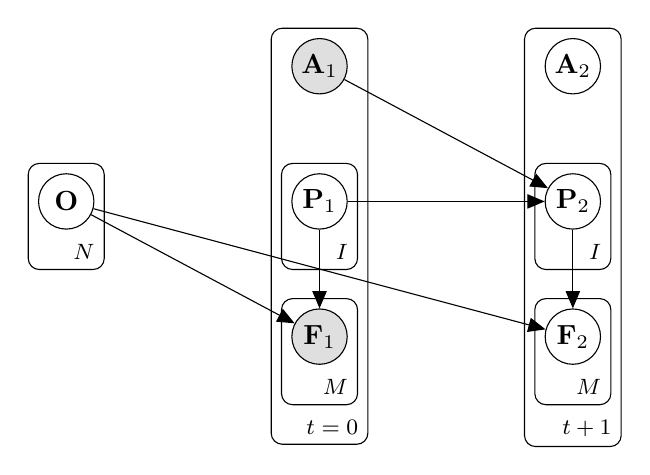
\begin{tikzpicture}
		% Define nodes
		\node[obs] (F) {$\SetOf{F}_1$};
		\node[latent, above=of F]  (P) {$\SetOf{P}_1$};
		\node[latent, left=of P, xshift=-1.5cm] (O) {$\SetOf{O}$};
		\node[obs, above=of P]  (A) {$\SetOf{A}_1$};

		\node[latent, right=of F, xshift=1.5cm] (F2) {$\SetOf{F}_2$};
		\node[latent, above=of F2]  (P2) {$\SetOf{P}_2$};
		\node[latent, above=of P2]  (A2) {$\SetOf{A}_2$};


	  % Connect the nodes
		\edge {P,O} {F};
		\edge {P2,O} {F2};
		\edge {P,A} {P2};

		% Plates
		\plate {pp} {(P)} {$I$}
		\plate {po} {(O)} {$N$}
		\plate {pf} {(F)} {$M$}

		\plate {pp2} {(P2)} {$I$}
		\plate {pf2} {(F2)} {$M$}

		\plate {} {(F)(P)(A)(pp)(pf)} {$t=0$}
		\plate {} {(F2)(P2)(A2)(pp2)(pf2)} {$t+1$}

	\end{tikzpicture}
	\end{center}


	We want to obtain the optimal action that will minimize the entropy over the posterior
	distribution:

	\Eq{  \arg\!\min_{A_{t+1}} H(\prob{\SetOf{O},\SetOf{P_{t+1}}|\SetOf{F_{1:t}},\SetOf{A_{t:t+1}}})}

	We can obtain this distribution by:

	\[
	\prob{\SetOf{O},\SetOf{P_{t+1}}|\SetOf{F_{1:t}},\SetOf{A_{t:t+1}}} =
	 \int \prob{\SetOf{O},\SetOf{P_{t+1}}, \SetOf{F_{t+1}}|\SetOf{F_{1:t}},\SetOf{A_{t:t+1}}} d\SetOf{F_{t+1}} =  
	\]

	\[
	\int \overbrace{\prob{\SetOf{O},\SetOf{P_{t+1}}|\SetOf{F_{1:t+1}},\SetOf{A_{t:t+1}}}}^\text{our posterior} \cdot \prob{\SetOf{F_{t+1}}|\SetOf{F_{1:t}}, \SetOf{A_{1:t+1}}} d\SetOf{F_{t+1}}
	\]

	where 

	\[
	\prob{\SetOf{F_{t+1}}|\SetOf{F_{1:t}}, \SetOf{A_{1:t+1}}} =
	\]
	\[
	\int \int \prob{ \SetOf{F_{t+1}}, \SetOf{O}, \SetOf{P_{t+1}}| \SetOf{F_{1:t}},\SetOf{A_{t:t+1}}} d\SetOf{O} d\SetOf{P_{t+1}}
	\]
	\[
	\int \int \overbrace{\prob{ \SetOf{F_{t+1}}|\SetOf{O},\SetOf{P_{t+1}}}}^\text{observation model} \cdot \overbrace{\prob{\SetOf{O},\SetOf{P_{t+1}}| \SetOf{F_{1:t}},\SetOf{A_{1:t+1}}}}^\text{action model} d\SetOf{O} d\SetOf{P_{t+1}}
	\]

	In our first implementation we assume the action model to be fully deterministic (delta function), so:

	\[
	\prob{ P_{t+1}|A_{t+1}, P_t} = \delta(p_{t+1})
	\]


\bibliographystyle{plain} 
\bibliography{literature}


% pdflatex pgm-mid-report.tex
% bibtex pgm-mid-report.aux
% pdflatex pgm-mid-report.tex
% pdflatex pgm-mid-report.tex
% open pgm-mid-report.pdf




\end{document}

